\documentclass{crypto-exercise}
\usepackage{amsthm}
\author{Sven Laur}
\contributor{Sven Laur}
\editor{Sven Laur}
\tags{ECB mode of operation, pseudorandom permutation, insecurity proof, block cipher mode of operation}

\newcommand{\COLL}{\mathsf{Coll}}
\newcommand{\ECB}{\textsc{Ecb}}
\newcommand{\FPERM}{\FFF_{\text{perm}}}
\renewcommand{\ADVIND}[2]{\ADV^{\mathrm{ind}}_{#1}(#2)}

\begin{document}
\begin{exercise}{Insecurity of ECB mode of operation}
A block cipher is commonly modelled as a $(t,q,\varepsilon)$-pseudorandom permutation family $\FFF$. As such, it is perfect for encrypting a single block. The electronic codebook mode $\ECB_f(m_1,\ldots,m_n)= (f(m_1),\ldots, f(m_n))$ uses a same permutation $f\gets\FFF$ for all message blocks. The latter is known to be insecure. Find an algorithm that can distinguish $\textsc{Ecb}_f:\MSPACE^n\to\MSPACE^n$ from a random permutation over $\MSPACE^n$. Is this weakness relevant in practise or not?
\end{exercise}
\begin{solution}
Let us first formalise the the indistinguishability of $\ECB_f$ form a random permutation in terms of two games. In the first game $\BGAME_0$, the adversary $\AD$ has an oracle access to the $\ECB_f(\cdot)$ function. In the second game $\BGAME_1$, the adversary $\AD$ has an oracle access to a random permutation $f:\MSPACE^n\to\MSPACE^n$. Corresponding games where $\FPERM$ denotes the set of all permutations over $\MMM^n$ are depicted below:
\begin{align*}
  \begin{game}{\BGAME_0^\AD}
    & f \gets \FFF\\
    & \RETURN \AD^{\ECB_f(\cdot)}
  \end{game}
  \qquad\qquad
  \begin{game}{\BGAME_1^\AD}
    & F \gets \FPERM\\
    &\RETURN \AD^{F(\cdot)}
  \end{game}
\end{align*}
The $\ECB_f$ is a $(t,q,\varepsilon)$-secure pseudorandom permutation if for all $t$-time adversaries who make at most $q$ function calls the distinguishing advantage is bounded:
\begin{align*}
\ADVIND{\BGAME_0,\BGAME_1}{\AD}=\abs{\pr{\BGAME_0^\AD=1}-\pr{\BGAME_1^\AD=1}}\leq\varepsilon\enspace.
\end{align*}

To show the insecurity of $\ECB$ mode of operation it is sufficient to contract an efficient adversary that has large distinguishing advantage. For that, let us define an adversary $\AD$ that makes a single oracle call for querying a message $\vec{m}=(m,m\ldots,m)$ and then outputs one if all blocks are the same:
\begin{align*}
\begin{fblock}{\AD^{\ORA(\cdot)}}
& (c_1,\ldots,c_n)\gets\ORA(m,\ldots,m)\\
& \IF \exists i,j: c_i\neq c_j \ \THEN \RETURN 0\\
& \ELSE \RETURN 1
\end{fblock}
\end{align*} 
If we substitute this definition into the games $\BGAME_0$ and $\BGAME_1$ we get simplified games:
\begin{align*}
\begin{game}{\GAME_0}
    & f \gets \FFF\\
    & c_1\gets f(m)\\
    & \ldots\\ 
    & c_n\gets f(m)\\
    & \IF \exists i,j: c_i\neq c_j \ \THEN \RETURN 0\\ 
    & \ELSE \RETURN 1
\end{game}
  \qquad\qquad
  \begin{game}{\GAME_1}
    & F \gets \FPERM\\
    & c_1\getsu \MSPACE\\
    & \ldots\\
    & c_n\getsu \MSPACE\\
    & \IF \exists i,j: c_i\neq c_j \ \THEN \RETURN 0\\ 
    & \ELSE \RETURN 1\enspace.
  \end{game}
\end{align*}
Note that we can replace the evaluation of $F(\vec{m})$ in the game $\GAME_1$ by random sampling of output components, since the random permutation evaluated on a single argument gives a random element form $\MSPACE^n$ as a reply. In the game $\BGAME_0$, a fixed permutation $f$ is evaluated on the same argument $m$  and consequently $c_1=\ldots=c_n$. As a result, we get \begin{align*}
\pr{\GAME_0=1}=1 \qquad\text{and}\qquad
\pr{\GAME_1=1}=\frac{1}{\abs{\MSPACE}^{n-1}}\enspace,
\end{align*}
from which we can conclude 
\begin{align*}
\ADVIND{\BGAME_0,\BGAME_1}{\AD}=1-\frac{1}{\abs{\MSPACE}^{n-1}}=\frac{\abs{\MSPACE}^{n-1}-1}{\abs{\MSPACE}^{n-1}}\approx 1 \quad\text{for}\quad n>1\wedge \abs{\MSPACE}>1\enspace.
\end{align*}
Since $\AD$ is very efficient algorithm, we can conclude that $\ECB$ mode of operation is not a $(t,q,\varepsilon)$-pseudorandom permutation for all practically relevant parameter values.

The scheme is vulnerable against practical attacks because the ciphertext leaks which plaintext blocks are identical. The effect is particularly pronounced when we encrypt images.

\begin{figure}[!h]
\begin{center}
\frame{
\includegraphics[width=5cm]{figures/tux}}
\frame{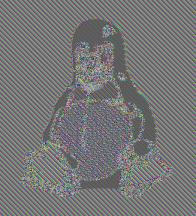
\includegraphics[width=5cm]{figures/tux-ecb}}
\frame{
\includegraphics[width=5cm]{figures/tux-secure}}
\end{center}
\caption{$\ECB$ mode of operation applied to an image file. Left pane is the original plaintext. The center pane is encrypted with the $\ECB$ mode of operation. The right pane is encrypted with secure pseudorandom  permutation defined on the entire image. Pictures are courtesy of Wikipedia}
\end{figure}
\end{solution}
\end{document} 
